%************************************************
\section{Task 2: Childproof} % (fold)
\label{sec:res_childproof_task}
%************************************************

%************************************************
\subsection{Question 0}\label{question2:0}
%************************************************
\emph{What level of understanding do you have at the moment about the SSM?}\\

The scale goes from 1 \emph{(Not at all)} to 7 \emph{(Expert)}.
\begin{table}[H]
	\begin{center}
		\small \begin{tabular*}{1.15\columnwidth}{lcccccr}
			\\ \hline \hline
			(1) & (2) & (3) & (4) & (5) & (6) & (7) \\ \hline \hline

		 	0 (0.0\%) & 1 (5.88\%) & 2 (11.76\%) & 4 (23.53\%) & 7 (41.18\%) & 2 (11.76\%) & 1 (5.88\%)\\ \hline
		\end{tabular*}
	\end{center}
\end{table}

\begin{figure}[H]
	\centering
	
\includegraphics[width=0.6\linewidth]{gfx/Chapter_EvaluationResults/ChildproofTask/question0}
\end{figure}
% section sec:question0 (end)

%************************************************
\subsection{Question 1}\label{question2:1}
%************************************************
\emph{Were you able to finish this task?}
\begin{table}[H]
	\begin{center}
		\small \begin{tabular*}{0.35\columnwidth}{lr}
			\\ \hline \hline
			Yes & No \\ \hline \hline

		 	16 (94.1\%) & 1 (5.9\%)\\ \hline
		\end{tabular*}
	\end{center}
\end{table}

\begin{figure}[H]
	\centering
	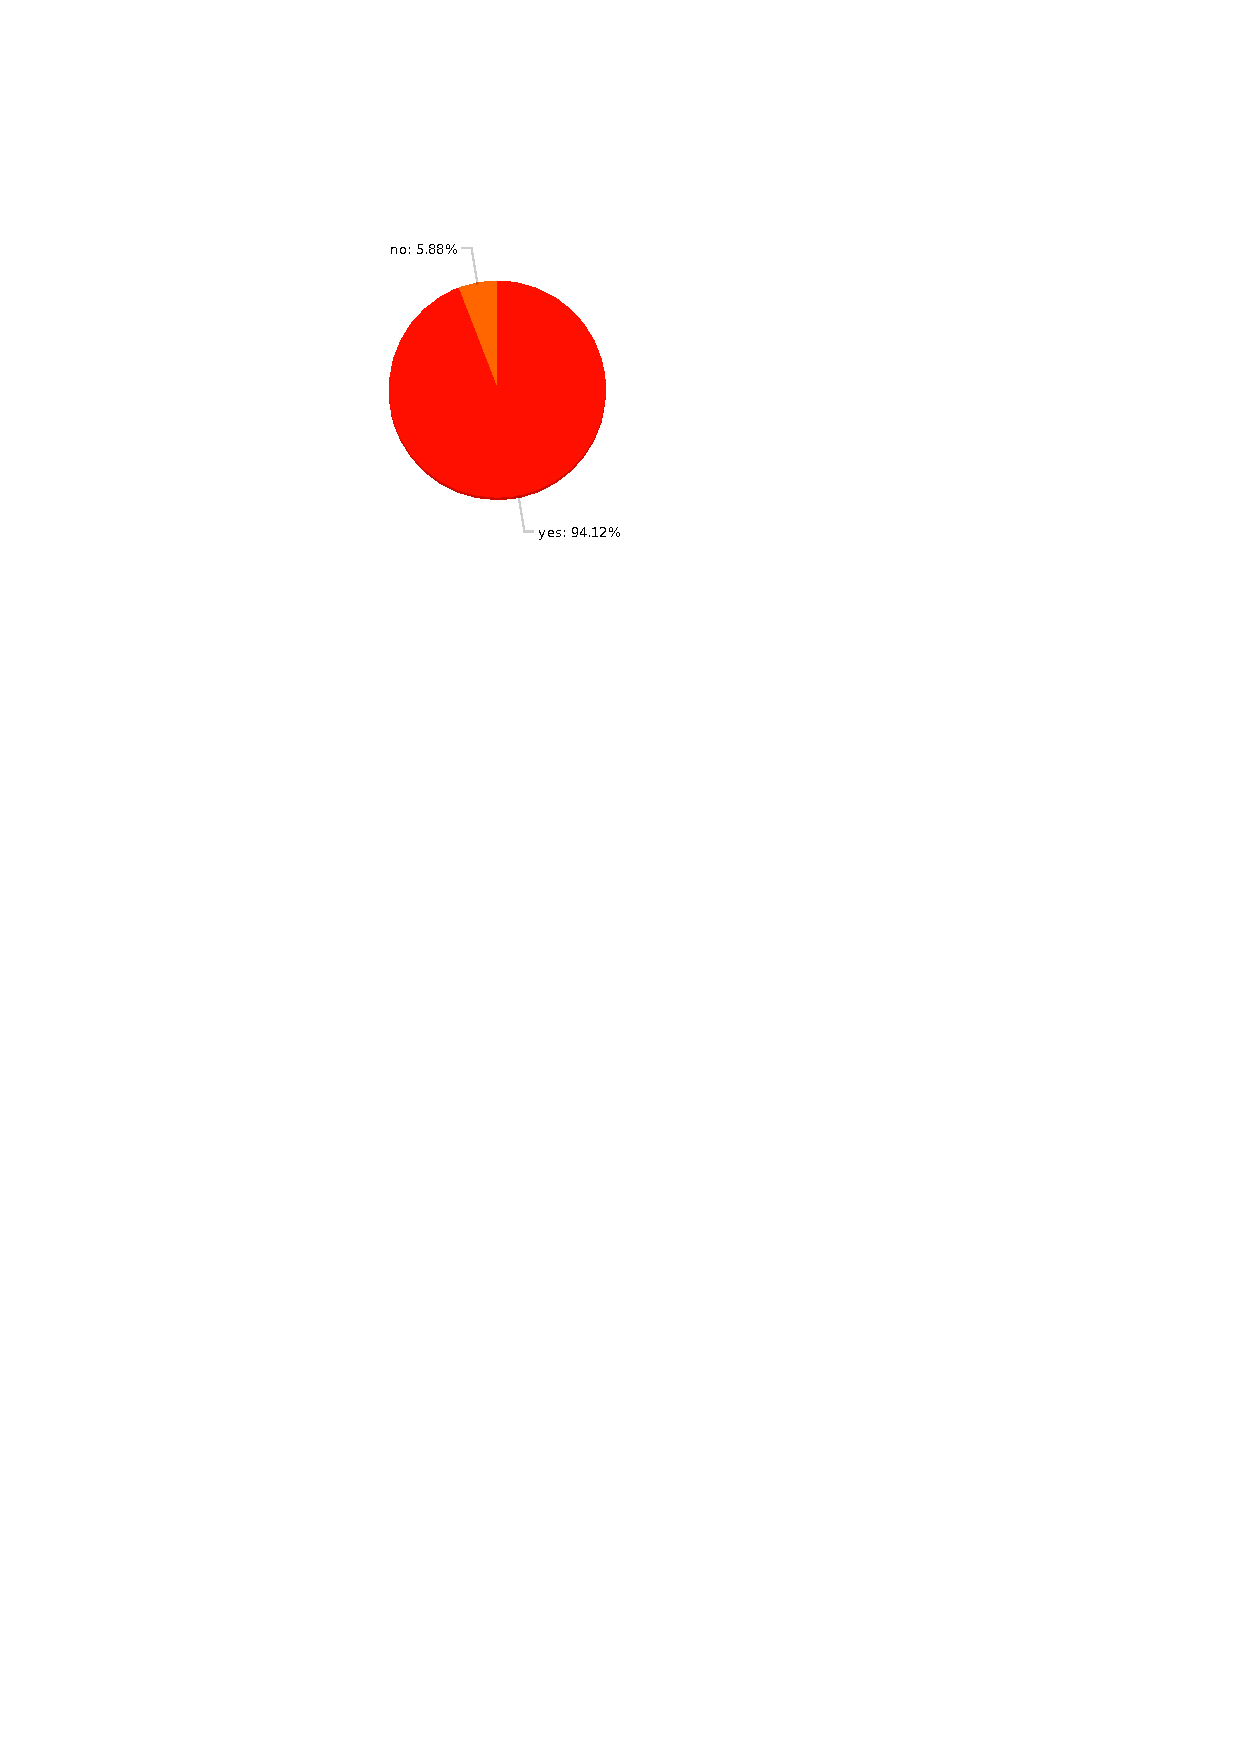
\includegraphics[width=0.5\linewidth]{gfx/Chapter_EvaluationResults/ChildproofTask/question1}
\end{figure}

\emph{If No, what difficulties have you come across that prevented you from finishing it?}
\begin{itemize}
	\item The objects I augmented with egocentric context data didn't show up in the spaces visualized in the client. I did notice some changes in the shading among the visualized spaces in the client, as I moved about, indicating that it might just be a matter of forgetting filling in a field somewhere as to the name of the objects or something like that. An indication of that things were actually classified correctly even if I couldn't see it is that It was possible to pick up the pen.
\end{itemize}
% section sec:question1 (end)

%************************************************
\subsection{Question 2}\label{question2:2}
%************************************************
\emph{Did you find this framework useful for simulating the situative space model?}
\begin{table}[H]
	\begin{center}
		\small \begin{tabular*}{0.35\columnwidth}{lr}
			\\ \hline \hline
			Yes & No \\ \hline \hline

		 	17 (100.0\%) & 0 (0.0\%)\\ \hline
		\end{tabular*}
	\end{center}
\end{table}

\emph{Why?}
\begin{itemize}
	\item Objects can be easily decorated with context information and interacting with them can be tested quickly because the framework takes care of basic interaction and movement in the space
	\item The simulation is very easy to understand and the increased usability makes it useful to prove the concept of how Context aware applications can be built.
	\item Very easy to set up and test a system behaviour where basic interactions are involved
	\item because with a few easy steps I was able to model the desired environment and got a notification api for free!
	\item well, just to walk around and see how objects were reclassified based on my orientation is worth something. it would have been nice to have the spaces visualized as spaces though, with animations that allow you track when objects transition from one space to another, and not as just as plain table entries.
	\item One can interact with designed objects.
	\item It was easy to use and It has a lot of possible utilities
	\item They can be close to realistic.
	\item Ease of naming objects and performing basic pick\_up interaction.
	\item Because I was able to complete the task and it involved setting up an unfamiliar to me. Besides, the presentation made me curious to try and implement functionality.
	\item It is very easy to import a ''scene'' and augment the objects with different information and interaction types.
\end{itemize}
% section sec:question2 (end)

%************************************************
\subsection{Question 3}\label{question2:3}
%************************************************
\emph{How easy/hard did you find the process of augmenting the objects to monitor?}\\

The scale goes from 1 \emph{(Very easy)} to 7 \emph{(Very hard)}.
\begin{table}[H]
	\begin{center}
		\small \begin{tabular*}{1.15\columnwidth}{lcccccr}
			\\ \hline \hline
			(1) & (2) & (3) & (4) & (5) & (6) & (7) \\ \hline \hline

		 	6 (35.29\%) & 7 (41.18\%) & 2 (11.76\%) & 0 (0.0\%) & 2 (11.76\%) & 0 (0.0\%) & 0 (0.0\%)\\ \hline
		\end{tabular*}
	\end{center}
\end{table}

\begin{figure}[H]
	\centering
	
\includegraphics[width=0.6\linewidth]{gfx/Chapter_EvaluationResults/ChildproofTask/question3}
\end{figure}
% section sec:question3 (end)

%************************************************
\subsection{Question 4}\label{question2:4}
%************************************************
\emph{How easy/hard did you find the usage of the framework as a whole?}\\

The scale goes from 1 \emph{(Very easy)} to 7 \emph{(Very hard)}.
\begin{table}[H]
	\begin{center}
		\small \begin{tabular*}{1.15\columnwidth}{lcccccr}
			\\ \hline \hline
			(1) & (2) & (3) & (4) & (5) & (6) & (7) \\ \hline \hline

		 	4 (23.53\%) & 7 (41.18\%) & 4 (23.53\%) & 0 (0.0\%) & 2 (11.76\%) & 0 (0.0\%) & 0 (0.0\%)\\ \hline
		\end{tabular*}
	\end{center}
\end{table}

\begin{figure}[H]
	\centering
	
\includegraphics[width=0.6\linewidth]{gfx/Chapter_EvaluationResults/ChildproofTask/question4}
\end{figure}
% section sec:question4 (end)

%************************************************
\subsection{Question 5}\label{question2:5}
%************************************************
\emph{What other parameters, if any, would you find useful for the system to monitor, besides proximity and visibility?}

\begin{itemize}
	\item Historical information about the agent: what actions has he performed so far, objects with which he has interacted with so far, etc
	\item How long an action can take. For example, a person can stay on the bad for ten hours. If the time is exceeded, a nurse should be informed.
	\item Depending on the application, it might be useful to monitor temperature, weight, etc.
	\item Previous interactions
	\item temperature, on/off state (outlet voltage), age (number of days the milk has)
	\item audio aspects of for instance the perception space.
	\item temperature, humidity, light.
	\item Temperature
	\item Orientation of certain objects. A computer screen might be close but you might be viewing it from behind.
	\item A useful parameter would be something linked to the user's perception of the existence of an object. For example, when you sit next to an open fire, you might not have a visual stimulus (let's assume you have your eyes closed) that confirms that objects presence; but rather you perceive its warmth. Thus, ''perceptibility'' could be defined as a measure of the subjects awareness of an object as any combination of feedback from his or her senses, in regard to said object.
	\item In the case of the childproof system: the height difference between the child and the outlet.
	\item weight, size, shape
\end{itemize}
% section sec:question5 (end)

%************************************************
\subsection{Question 6}\label{question2:6}
%************************************************
\emph{What information, besides what's already served, do you think that should be available through the API?}

\begin{itemize}
	\item List of objects the agent has interacted with... or maybe last X objects
	\item I'd make available all the parameters, see previous answer.
	\item the distance between all objects, so that we can have more than a visual map. Distance from edges.
	\item some constraints that can be set for a specific object
	\item Depends on who is using the API. If it is a software programmer, no. If it is a user with technical abilities who has to simulate different scenarios it is close to enough.
	\item On/Off state for objects; for example a door can be locked or unlocked, a faucet might be on/off. 
\end{itemize}
% section sec:question6 (end)

%************************************************
\subsection{Question 7}\label{question2:7}
%************************************************
\emph{What types of interaction, besides pick up/put down, do you find absolutely necessary to make the simulator more realistic?}

\begin{itemize}
	\item Dropping an object at current location
	\item If a person takes his pills, it can not be simulated right now. The fact that an electronic device is turned on/off.
	\item Push, pull action (for outlets for example).
	\item Custom actions depending on the type of object.
	\item Possibility to increase speed for interactions
	\item There could be state change notifications. Or even surroundings aware interaction: light goes on in a room you are entering, etc.
	\item different types of usages of the objects (for the piano, the laptop,...)
	\item touch / press / push / pull
	\item turn off, on (electronics, water tap, shower)
	\item simulation of mediators (keyboards, displays, etc.)
	\item for the simulation that was enough
	\item Drag, rotate
	\item for me it's realistic enough
	\item I think pull, push for objects
	\item if a standard on/off state could be added, a turn on / turn off action might be useful
	\item A generic USE action would help is many situations as many objects that are interacted with might have a main USE method. pickup/putdown could be specific implementations of use.
	\item An interaction leads to an operation. A possible redesign of this feature would be adding an intermediary abstraction that is related to the scope of the operation on the object. An internal operation could be implemented in the object that is manipulated (use the pen to write), while an external interaction would result in an operation that changes the object's context in relation to other objects (moving the pen around).
	\item Any form of custom action that depends on the object you interact with. Some of the objects in Task1 had this sort of behaviour: you were able to play the piano, you were able to read mail on the laptop, you were able to pour tea
\end{itemize}
% section sec:question7 (end)

%************************************************
\subsection{Question 8}\label{question2:8}
%************************************************
\emph{Please provide any ideas to improve this framework! (also point out bugs you might have found, things that you liked, etc)}

\begin{itemize}
	\item Not sure how it is implemented right now but I can imagine such a simulation being a multiple step process: 1. the simulation being built by some developers. 2. After it has been developed, it is given to some ''experts'' which calibrate the simulation so that it better simulate the reality of the situation it was designed for. For this they would need to easily change (possibly even at runtime) some attributes of the EgocentricContextData like: perception distance, recognition distance, examination distance, for any of the augmented objects. The framework should allow for this... I think.
	\item I liked the framework. Easy to use.
	\item Extend it to provide a more complete range of actions.
	\item It is very easy to use and identify the monitored objects.
	\item No bugs found in the evaluation.
	\item I really liked the idea and other than the fact that I did not find how I can use lastMeasuredDistance meaningfully, I have no other observations. Really nice work!
	\item physics model, no gravity,
	\item there are some SSM entity type naming issues that could be improved. e.g. the term ''surface'' might not be appropriate for all objects that can accept an object (e.g. the sink).
	\item regarding bugs, I couldn't complete task 2. it is probably not a bug but the lack of providing some info that was needed. Maybe the instructions for task 2 could be a notch clearer (e.g. with examples for how the field should look when filled in for the sockets and for the pen).
	\item first impression is that it's easy to use and friendly. The Add User Data part without help would have been a bit tricky, if that can be made easier. SceneExplorer Window a bit too heavy. Other that that, great.
	\item Trim the context variable for space EGOCENTRIC\_CONTEXT\_DATA
	\item Didn't noticed any bugs and I liked the fact that I had a different perception when I was a child than when I was an adult
	\item No bugs! As a first time usage it went fine!
	\item A potential weakness of this framework would be the lack of information regarding the relationship between objects. In this example, the child may pick up and pen and attempt to stick it the outlet. Is is trivial to conceive a logic that may cause the power in the outlet to shut down, preventing the kid from getting electrocuted (pen is selected, outlet is in action space). However, if the kid releases its grip on the pen, the system will register that both objects are in the action space, thus turning the power back on. If the kid then touches the pen, it will be too late to react as the child is already in danger of electrocution. A possible solution to this scenario could be adding a space that describes the interaction between two objects. A flower pot and the table it is placed on interact, though not in a way that is relevant to a child's safety. However, a pen stuck in an outlet may cause an interaction where a specific handling is necessary. The situation where the outlet is not in the action space as some electrical appliance may already be plugged in should be considered. The system should not react to the pen holding child's proximity to the already used outlet. The presence of an object in the action space can thus depend on how the said object interacts with other objects. Various object states may be needed in order to correctly simulate the above mentioned scenario
	\item It is very easy to augment objects with data. Would be nice if people could declare their own type of interactions.
\end{itemize}
% section sec:question8 (end)

%************************************************
\subsection{Question 9}\label{question2:9}
%************************************************
\emph{Given the SSM sets, what should be the condition for the SOS service to shut the electricity down in the outlets? Feel free to write the condition in simple words, pseudo-code or any language of your choice.}

\begin{itemize}
	\item if (pen is in selected space) and (outlet is in examinable set) then shut-down electricity for current outlet
	\item If outlet in actionSet and I am a kid, shut electricity down. But a kid runs a lot, the electricity may be shut down very often for no good reason, but to change the condition to selectedSet may be too late.
	\item Height of the agent should be under a limit (to consider a child) and the proximity to the outlet is less than 5 cm. Turn them on when proximity is greater than 1 m.
	\item if ((actionSpace.contains(outlet)) and (selectedSpace.contains(pen)) outlet.shutdown()
	\item If a child is approaching the outlet and has entered the Action Space with an item in the Selected Space the power should be cut off. Of course it also might raise the question if it is necessary to have something in hand. If the Outlet is not used, I think that power can be cut off just if the child is in the Action Space.
	\item the child holds has picked up the pen and the proximity to the outlet is small
	\item distance to pen <= actionable distance of the outlet (pen is inside of the outlet's ActionSpace)
	\item if (pen in kid\_human.hand) outlets.shut\_down
	\item if pen is in the manipulated set and socket is in examinable set then turn off electricity
	\item shut down the power if the child is at 2 m from the socket
	\item If the user has something in hand (define small object) and moves towards the outlet, when reaching the limit of 1 meter and has the pen at hand, disable the outlet.
	\item When the child is in the Action Space with an object from the Manipulated Set, show an alert, play a sound and shut the electricity.
	\item assuming we can set callbacks on any set modification:
	\item The pen has to be in the selection space and the outlet in the use space.
	\item in case the distance between the child and the outlet is smaller than a given delta, the electricity should be shut down.
	\item dangeous\_objects = set(has\_sharp\_edges(obj) for obj in all\_objects). If any(dangerous\_objects.intersection(selectedSet)) and any(outlets.intersection(actionSpace)): shut\_down\_electricity()
\end{itemize}
% section sec:question9 (end)

%************************************************
\subsection{Question 10}\label{question2:10}
%************************************************
\emph{Can you think of any system that could use the SSM sets and classification algorithms as building blocks? Please describe it shortly.}

\begin{itemize}
	\item A friendship network with several kind of relationships and different possible interactions accordingly.
	\item Any home to help out with certain defined tasks e.g,: elder's home, persons with disabilities to help with daily activities or in case of urgencies. Hospitals. Public institutions guide a person from entrance to the needed assitance
	\item  Assistance for the visually impaired.
	\item  This system could be implemented for people with disabilities, especially visually impaired persons, to offer a augmented representation of their environment.
	\item  A tourist map that is context aware and can recommend places to visit that are near the current location, that are for example still open (maybe it's night, you don't want recommendations for a zoo), etc...
	\item  It would be fun to model the International Space Station with SSM. Think no gravity (physics engine for jMonkey?), resource management.
	\item  future bodyworn computer systems, starting with today's cellular phones.
	\item  provide help for people with disabilities
	\item  Any monitoring system, learning systems.
	\item  A kindergarten construction. It can be used to simulate all the possible places a kid can explore and possible things he can do.
	\item security application: auto-lock my computer screen when it's disappears from the intersection of my Examinable Set and Action Space (or perhaps just action space)
	\item Automatic light switching based on the position of the inhabitant of a home (not motion-based). This can be generalized to a system that defines custom operation modes of devices in a home, depending on what the user is doing.
\end{itemize}
% section sec:question10 (end)

% section sec:res_childproof_task (end)